\documentclass[11pt, titlepage]{article}
\usepackage[a4paper, nomarginpar, total={170mm,257mm}, left=40mm, right=25mm, top=20mm, bottom=20mm]
{geometry}

\title{Nekilnojamojo turto kainų pokyčiai Lietuvoje 2009-2019m.}
\author{Gabrielė Gatulytė}
\usepackage[utf8]{inputenc}
\usepackage[L7x]{fontenc}
\usepackage[lithuanian]{babel}
\usepackage{graphicx}
\usepackage{float}
\usepackage{setspace}
\onehalfspacing
\usepackage{indentfirst}
\usepackage{hyperref}
\hypersetup{
colorlinks=true, 
linkcolor=blue,
filecolor=blue,
urlcolor=blue,
citecolor=red
}


\usepackage[
backend=biber, style=apa, url=false
]
{biblatex}
\addbibresource{saltiniai.bib}

\begin{document}
\maketitle
\tableofcontents
\newpage

\section{Įvadas}
\subsection{Nekilnojamojo turto samprata ir klasifikavimas}
Nuo pat senų laikų nekilnojamasis turtas yra vertinamas kaip viena pelningiausių investavimo sričių. Skirtingose šalyse nekilnojamasis turtas suprantamas nevienodai. Daugelyje šalių nekilnojamasis turtas yra suvoktinas kaip žemė. Pavyzdžiui, Ekonomikos terminų žodyne nekilnojamojo turto sąvoka taip pat yra susiejama su žeme: „Nekilnojamas turtas - pagal prigimtį nejudinamas daiktas, t. y. žemė ir su ja susiję objektai, kurių negalima perkelti į kitą vietą nesumažinant jų vertės ar nepakeičiant paskirties ir formos”. \parencite{galiniene2011ekonomikos}
\par
Pirmiausia, NT yra skirstomas į dvi pagrindines grupes – gyvenamosios paskirties ir negyvenamosios paskirties turtą. Šiame rašto darbe didesnis dėmesys bus skiriamas gyvenamosios paskirties pastatams. 
\begin{figure} [H]
\center
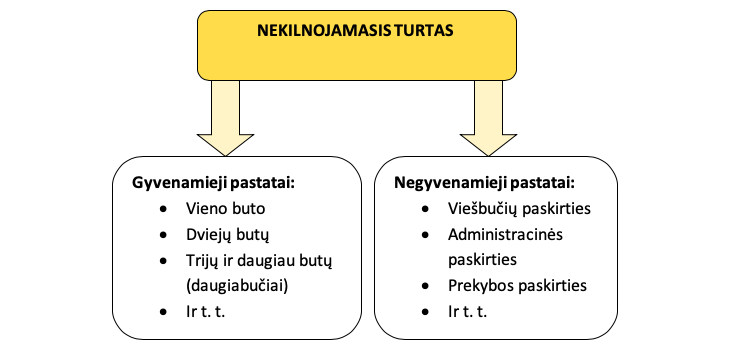
\includegraphics[scale=0.5]{toks}  
\caption{Nekilnojamojo turto klasifikavimas}
\end{figure}                        
\subsection{Veiksniai įtakojantys nekilnojamojo turto rinkos kainas}
Čia vertėtų pradėti nuo sąvokos, kas yra rinka, pavyzdžiui, literatūroje rinka apibūdinama kaip: „Terpė, kurioje vyksta prekių ir paslaugų mainai, pasitelkus kainų mechanizmą” \parencite{tupenaite2009nekilnojamojo}. Tačiau, kad galėtų vykti tokie mainai būtinos bent dvi rinkos veikėjų grupės: pirkėjai ir pardavėjai. Kiekvienas rinkos dalyvis tiek, kuris parduoda, tiek, kuris perka nekilnojamąjį turtą siekia sau maksimalios naudos, kaip sakė A. Smitas: „Kiekvieno pirštai linksta į save“.  Tad, tiek pirkėjo, tiek pardavėjo lūkesčiai daro įtaką nekilnojamojo turto kainai, nes nuo jų veiksmų priklauso sandorio eiga. 
\par
Žinoma, NT vertė priklauso ir nuo nekilnojamojo turto savybių, kurios lemia norimo nusipirkti turto patrauklumą. Vis dėl to, didžiausia įtaką kainai turi mikro lygmens veiksniai, tokie kaip teisiniai dokumentai, mokesčių sistema, palūkanų normos ir galimybės gauti paskolą, tačiau taip pat nepamirškime ir infliacijos, darbuotojų užimtumo lygio, atlyginimų dydžio, gyventojų skaičiaus kitimo. 
\section{Nekilnojamojo turto pokyčių analizė}
\subsection{Nekilnojamojo turto kainų apžvalga}
Verta pabrėžti, kad namų kainų spartus didėjimas pradėtas fiksuoti nuo 2002m. Toks spartus naujų namų ir butų kainų kilimas siejamas su bendru Lietuvos ekonomikos augimu, kasmet sukuriant 8-9\%. BVP. Didžiausias nagrinėjamu laikotarpiu kainų pokytis nustatytas 2008m., kai Lietuvą bei visą pasaulį ištikusi ekonominė krizė palietė nekilnojamojo turto rinką: išaugo gyventojų pajamos, kurios išprovokavo statybų bumą ir dėl to ženkliai kilo nekilnojamojo turto kainos. 2009m. nekilnojamojo turto rinkos aktyvumas buvo mažiausias per šešerius metus būsto kainos mažėjo 13,8\% lyginant su prieš tai buvusiais metais. 2010m. antroje metų pusėje pradėti fiksuoti teigiami butų kainų pokyčiai. 2015m. nekilnojamojo turto rinka buvo mažiau aktyvi nei 2014m. Pavyzdžiui, 2015m. sudarytų butų pirkimo-pardavimo sandorių buvo 9,8\% mažiau nei lyginant su 2014m. Visgi 2018m. NT rinka Lietuvoje trečius metus iš eilės buvo savo aktyvumo viršūnėje - nuosaikus registruotų sandorių augimas buvo fiksuojamas butų ir individualių namų segmentuose. 
\par
Kalbant apie kainas 2019m. tai neseniai išleistoje Lietuvos banko apžvalgoje nurodoma, kad 2019m. Lietuvos ekonomika augs lėčiau. \href{https://www.lb.lt/uploads/publications/docs/21756_d778713ca234ccc09dc70e7312b44d89.pdf}{Lietuvos banko apžvalga}
Keletas iš priežasčių, kas sąlygos ekonomikos lėtėjimą: darbuotojų trūkumas bei atlyginimų didėjimas, gyventojų perkamosios galios didėjimas ir sumažėjęs investicijų augimas. Vis dėl to, Lietuvos ekonominė situacija išlieka palanki būsto rinkos augimui, tačiau tam reikalingi taip pat palankūs išoriniai faktoriai. Būsto paskolų palūkanos tebėra santykinai nedidelės, o gyventojų pajamos toliau sparčiai auga, todėl būsto įperkamumas ir galimybės gauti paskolą - gerėja. Didėjantis namų ūkių optimizmas dėl ateities perspektyvų suaktyvino ir vartojimo paskolų segmentą, 2018m. tokių paskolų portfelis padidėjo 8,7\% Tikėtina, kad šalies ekonomikai augant, panašios tendencijos turėtų išsilaikyti ir toliau. 
\subsection{Nekilnojamojo turto kainų pokyčius lėmusių veiksnių apžvalga}
Analizuojant nekilnojamojo turto sektorių matyti, kad jo vaidmuo yra labai reikšmingas ne tik Lietuvai, bet ir kiekvienam žmogui. NT sektoriaus veiklos rezultatai dėl plačiai išvystytų materialinių ir finansinių santykių, formuojančių kitų vietos rinkos prekių ir paslaugų paklausą, turi didelė reikšmę ekonomikai ir prekybai.\parencite{simanavivciene2011makroekonominiku} Kylant gyvenimo lygiui žmonės ieško geresnės kokybės bei didesnių būstų, o tai turi teigiamos įtakos paklausai, tačiau gimstamumas, gyventojų mažėjimas gali sumažinti nekilnojamojo turto ateities perspektyvas. Vienas iš pagrindinių faktorių, nulemiančių nekilnojamo turto rinkos vystymąsi, yra demografinės tendencijos. Visų pirma vertėtų apžvelgti pagrindinius demografinius rodiklius Lietuvoje: gyventojų skaičių, jų užimtumą bei tarptautinę migraciją. 
Kadangi Lietuva yra palygintai maža valstybė, tai gyventojų skaičius Lietuvos ekonomikai daro nemažą įtaką. Lietuvoje gyvenančių gyventojų skaičiaus dinamiką šalyje atspindi  \ref{fig:Rplot1} paveikslas.
\begin{figure}[H]
\center
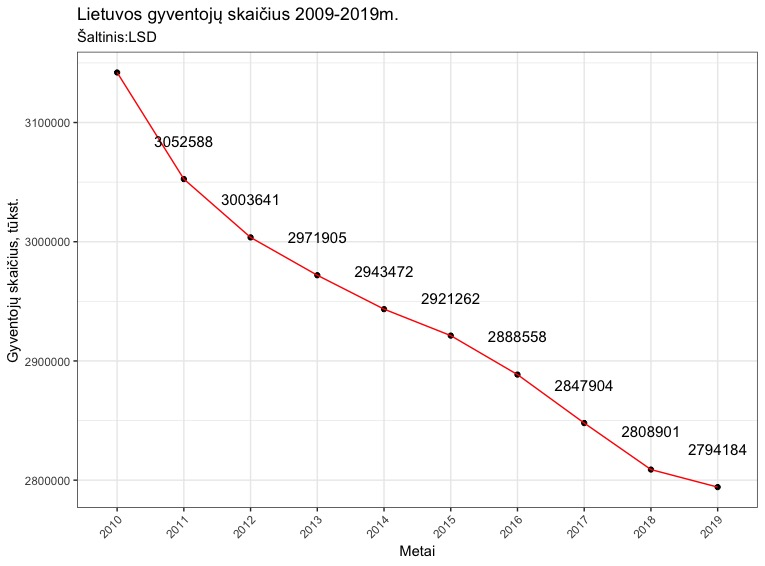
\includegraphics[scale=0.5]{Rplot1}
\caption{Lietuvos gyventojų skaičiaus dinamika}
\label{fig:Rplot1}
\end{figure}
\par 
Lietuvos statistikos departamento šaltinis nurodo, kad šalies gyventojų skaičius nuolat mažėja. Veiksniai, kurie gali daryti įtaką šitokiam mažėjimui tai gyventojų emigracija iš Lietuvos, neigiama natūrali gyventojų kaita, taip pat verta paminėti kad ir Lietuvos mirtingumo lygis pastaraisiais metais yra vienas aukščiausių Europos Sąjungoje.  Vis dėl to, didesnį dėmesį norėčiau skirti emigracijai žr. \ref{fig:Rplot2} pav. 
\begin{figure}[H]
\center
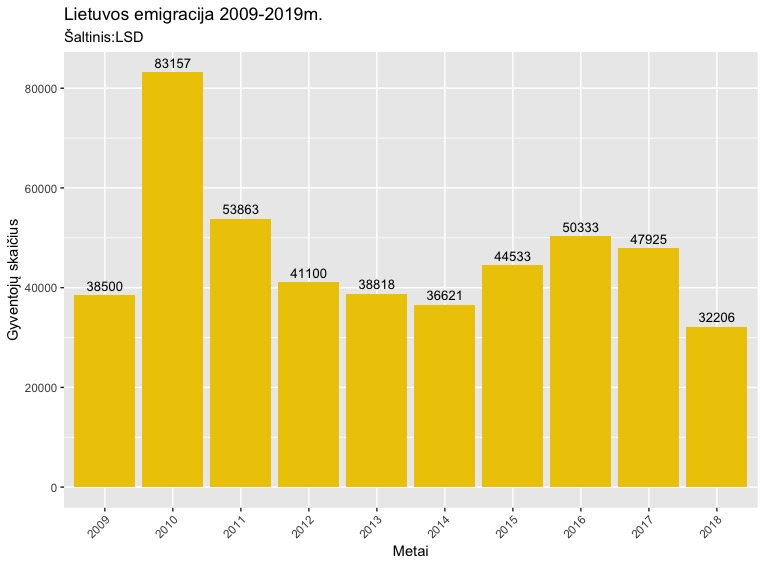
\includegraphics[scale=0.5]{Rplot2}
\caption{Emigracija Lietuvoje nuo 2009m. }
\label{fig:Rplot2}
\end{figure}
\par
Šitoks didelis skaičius emigrantų daro įtaką nekilnojamojo turto rinkai. Anot, Lietuvos nekilnojamojo turto agentūros asociacijos (LNTAA) valdybos nario Manto Mikočiūno: “Daugiausiai Lietuvoje būsto nuperka 25-45 amžiaus žmonės, tačiau ši piliečių grupė dažniausiai ir emigruoja. Tie, kurie nusprendžia grįžti į tėvynę, dažniausiai grįžta į didesnius miestus, o tai mažuosiuose miestuose ar provincijose sparčiai mažina perkamąją galią.” Taip pat, analizuojant atskirus miestus matyti, kad nuo 2013m. gyventojų skaičius augo tik Vilniaus mieste, visur kitur jis po truputį mažėjo. 
\subsection{Pagrindinių makroekonominių rodiklių apžvalga}
Nagrinėjant nekilnojamojo turto ir statybos sektoriaus svarbu atsižvelgti į bendrą Lietuvos ir pasaulio ekonomikos lygį ir jos vystymosi tendencijų prognozes. Kadangi vienas iš pagrindinių rodiklių, rodančių šalies išsivystymo lygį yra BVP, verta pirmiausia apžvelgti šio rodiklio dinamiką. \ref{fig:Rplot3} pav.
\begin{figure}[H]
\center
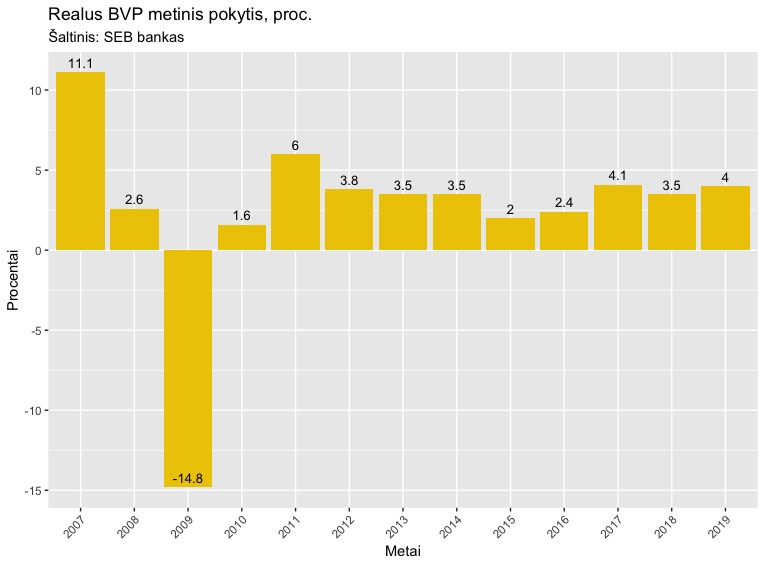
\includegraphics[scale=0.5]{Rplot3}
\caption{Realus BVP metinis pokytis (proc.) }
\label{fig:Rplot3}
\end{figure}
Ekonominės krizės laikotarpiu 2009 m. Lietuvos BVP nukrito iki 14,9 proc. Tai pirmasis metinis BVP kritimas nuo 2000-ųjų. Nuo 2009m. Lietuvos BVP tai kilo, tai nežymiai krito. 2019m. pateiktas 4,0 BVP yra tik I ketv. Neseniai Lietuvos bankas paskelbė, kad realusis BVP  2019m.  didės iki 3,2\%, na, o 2020m BVP prognozė bus kiek mažesnė tik iki 2,4\%.  Tačiau, kodėl kylantis BVP yra svarbus NT rinkai? Nes skatina nekilnojamo turto kainų didėjimą ir paprastai augant ekonomikai auga žmonių perkamoji galia, lūkesčiai, didėja kreditavimas. Tai didina nekilnojamo turto paklausą. Augant BVP galima tikėtis bazinių palūkanų normos didinimo. Centrinis bankas, didindamas bazines palūkanų normas apsaugo ekonomiką nuo perkaitimo bei reguliuoja infliacijos lygį. Infliacija taip pat yra svarbus reiškinys, \ref{tab:my-table}  lentelė, nes padidėjusi infliacija gali sumažinti pirkėjų perkamąją galią bei priversti centrinius bankus reaguoti ir kelti palūkanų normas. Gyventojams gali pradėti didėti įmokos už nekilnojamąjį turtą, o brangstant būtinosioms vartojimo prekėms ir paslaugoms gali likti vis mažiau galimybių sutaupyti. 2019m. infliacija sieks 2,3\% tad vis dėl to, atsižvelgiant į istorinį kontekstą, kol infliacija yra žemiau 5\% ribos, panikuoti neverta. 
\par
\begin{table}[H]
\begin{tabular}{|l|c|c|c|c|c|c|c|c|c|c|}
\hline
\textbf{Metai}  & 2013 & 2014 & 2015 & 2016 & 2017 & 2018 \\ \hline
\textbf{Vidutinis metinis SKVI pokytis (proc.)} & 1,2 & 0,2 & -0,7 & 0,7 & 3,7 & 2,5 \\ \hline
\end{tabular}
\caption{Vidutinė metinė infliacija pagal SKVI (proc.)}
\label{tab:my-table}
\end{table} 
\par
Kitas veiksnys į kurį reikėtų atkreipti dėmesį tai nedarbo lygis \ref{fig:Rplot4} pav.  Nedarbo lygis ir BVP yra glaudžiai susiję ekonomikos rodikliai: kuo daugiau darbuotojų, tuo daugiau paslaugų ir produkcijos ekonomika gali pagaminti. \parencite{azbainis2011pereinamojo}   Augant nedarbui greičiausiai išvysime  BVP mažėjimą. Visgi, BVP rodiklis atspindi praėjusių kelių mėnesių ekonominę situaciją. Tuo tarpu nedarbo lygis nurodo esamą ekonomikos būklę. Taigi, jeigu nedarbo lygis didėja, nekilnojamojo turto kainos mažėja bei atvirksčiai, nedarbo lygiui mažėjant kainos didėja.  Vertėtų pridėti, kad NT kainai įtakos turi ir vidutinis gyventojų atlyginimas, nes jeigu jis didėja, tai taip pat didėja ir nekilnojamojo turto kainos. 
\begin{figure}[H]
\center
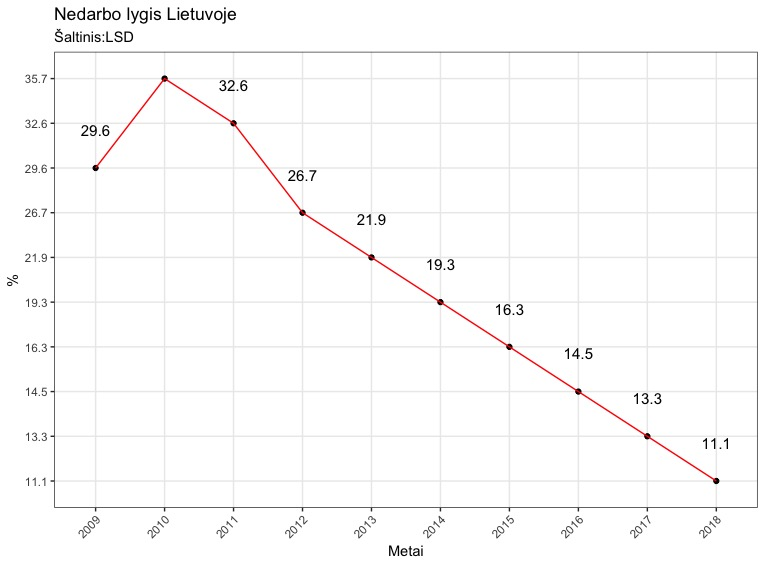
\includegraphics[scale=0.5]{Rplot4}
\caption{Nedarbo lygis}
\label{fig:Rplot4}
\end{figure}
\newpage
\section{Išvados}
Taigi, galime padaryti išvadą, kad  nekilnojamasis turtas, jo vertė ir rinkos pokyčiai turi didelę įtaką šalies ekonomikai. Nekilnojamasis turtas per gamybą ir vartojimą prisideda prie bendrojo vidaus produkto kūrimo, t.y. prie šalies ekonomikos stiprinimo. \parencite{galiniene2011ekonomikos} Taip pat, kalbant apie NT, yra daugelis veiksnių, kurie daro įtaka nekilnojamojo turto kainoms, keletas iš jų tai infliacija,nes infliacijos metu nekilnojamojo turto vertė įprastai didėja, palūkanų norma, nedarbo lygis, migracija, nuomos kaina, taipogi išoriniai įtakos veiksniai: ekonominiai, socialiniai ir politiniai. Lyginant naujos ir senos statybos būstus, tai kainų kritimui atsparesni yra senos statybos būstai.  Pasak ekonomisto dr. T. Šarapovo, tokio būsto pardavėjai linkę ilgiau palaukti pirkėjo, o naujų nekilnojamo turto projektų vystytojams „laikas turi aiškesnę kainą“ todėl jie linkę greičiau parduoti savo turtą.  Visgi, nors ir paskutinio metu NT kainos išlieka stabilios, tačiau stabilumo tendencija, vis dėlto, netruks labai ilgai: 2020m., ženkliai sumažėjus ES paramos apimtims, galimas gamybos apimčių mažėjimas, tada NT kainos priklausys nuo pačios Lietuvos ekonomikos, jei eksportas augs ir gamybos apimtys nemažės – tai didelių kainų pokyčių nebus, o priešingu atveju anot dr. T. Šarapovo,  galime tikėtis “didelių kainų šokų.”
\newpage
\nocite{*}
\printbibliography[title={Literatūra}]
\end{document}
